\section{The Dynamical Instability of Accumulated Correctness}

\subsection{Overview}

\S{}6 showed that knowledge cannot substitute for intelligence. This section derives a stronger dynamical consequence:

\begin{quote}
Accumulated correctness does not stabilize intelligence. It destabilizes it.
\end{quote}

The claim is not psychological. It does not say that knowledgeable people become unstable. It says that correctness, when reused in an inferential network, increases connectivity and therefore increases the branching structure of inference.

\subsection{Why correctness increases connectivity}

A proposition treated as correct becomes reusable. It can serve as a premise, connect to other propositions, generate consequences, support analogies, and become a node in further inquiry.

In IFGT vocabulary, accumulated knowledge increases local information density:
\[
I(s)\uparrow.
\]
But because correct propositions are reusable, this increase in \(I\) is not merely static. It increases the branching degree of information flow:
\[
\nabla\cdot J \uparrow.
\]

The more correct stopping structures a system accumulates, the more inferential paths become available.

\subsection{Why correctness contains no stopping condition}

Correctness does not stop inference. It justifies further inference.

If a proposition \(p\) is correct, then several questions become structurally legitimate: why is \(p\) correct, where does it apply, what are its exceptions, how does it relate to other correct propositions, and what follows from it?

Thus correctness functions as a branching source:
\[
\mathrm{correctness}(p)\Rightarrow \nabla\cdot J|_p\neq 0.
\]
The state \(\nabla\cdot J=0\) cannot be maintained around a proposition that remains reusable as correct.

\subsection{Branching explosion}

The structural chain is:

\begin{enumerate}
\item correct knowledge accumulates;
\item inferential connectivity increases;
\item branching degree increases;
\item stopping points dissolve.
\end{enumerate}

If the number of accumulated correct nodes is \(|V|\), then possible edges may grow approximately as \(|E|\sim |V|^2\). If a typical branching factor is \(b\), then paths to depth \(d\) grow as \(b^d\). The result is a regime in which no path can claim finality internally.

\subsection{Why ``more intelligence'' does not solve the problem}

The natural response to branching explosion is to add more intelligence: more knowledge, faster reasoning, deeper specialization, or larger search. Structurally, these responses do not remove the problem. They accelerate it.

More knowledge increases \(I\). Stronger reasoning increases branching degree. Faster processing compresses the time scale of the explosion without changing its structure. Specialization localizes the explosion but does not eliminate it.

The problem is therefore not insufficient ability. It is the absence of an internal stopping operator.

\begin{figure}[H]
\centering
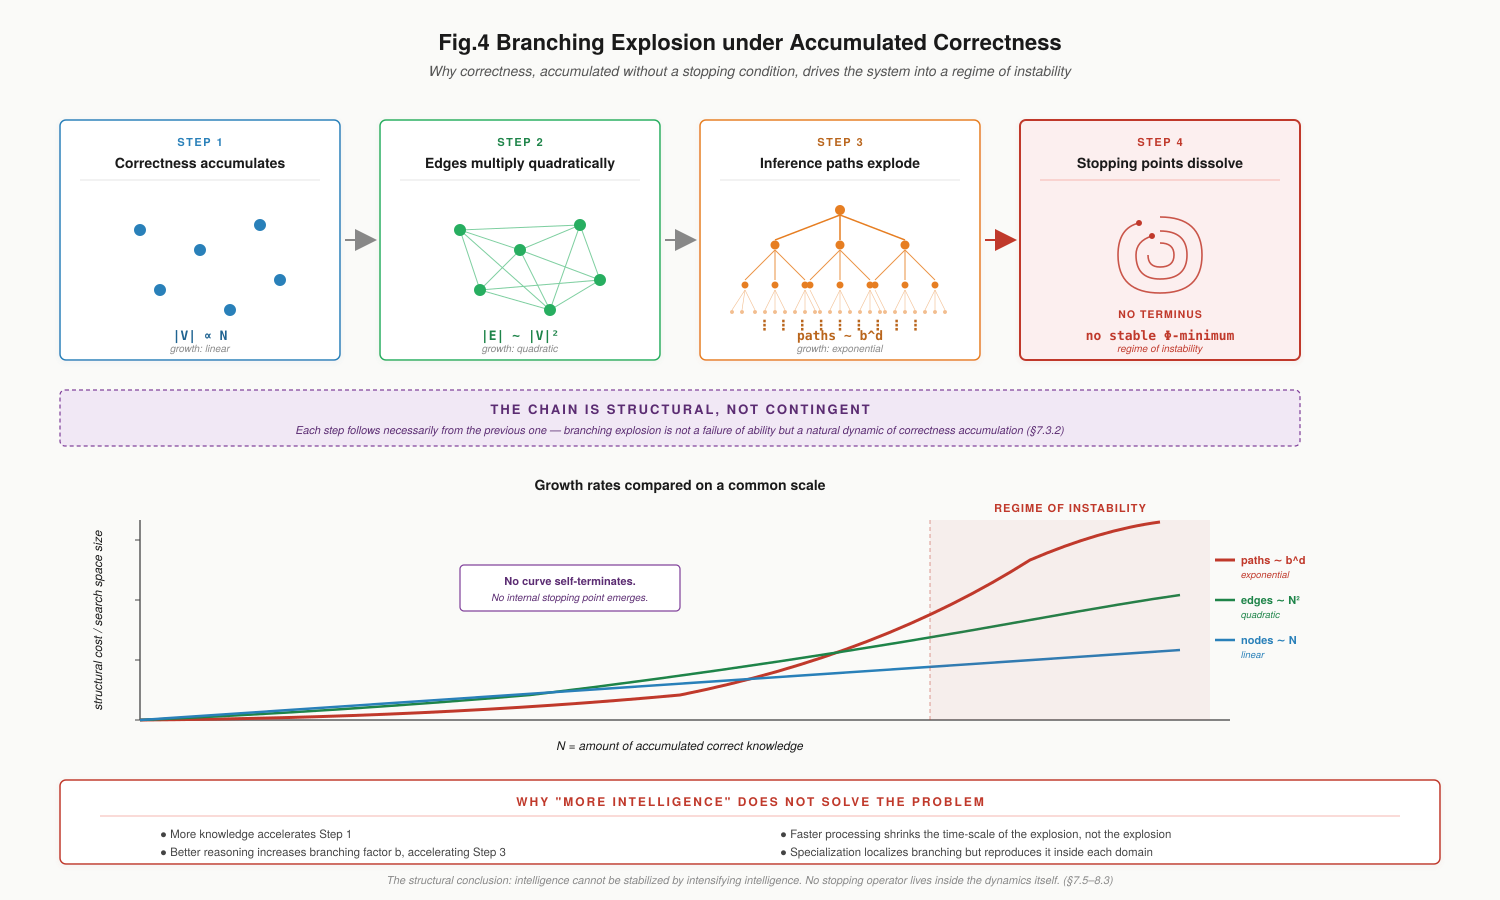
\includegraphics[width=\textwidth]{figures/fig4_branching_explosion.png}
\caption{Branching explosion under accumulated correctness. Correctness increases reuse, reuse increases connectivity, and connectivity dissolves internal stopping points.}
\label{fig:intelligence_part1_4}
\end{figure}

\subsection{Summary}

\begin{quote}
Correctness is not a stabilizer of intelligence. Correctness is a source of further inference. Accumulated correctness therefore produces branching explosion unless an externalized stopping structure intervenes.
\end{quote}
